A large challenge in applying standard manipulation and planning techniques to
deformable object manipulation is that of tractable modelling. Deformable object 
are often characterized by high-dimensional, continuous state-action spaces. Model-based 
planning has yet to scale up to the task of efficient planning in this
setting.

Recent work have gained traction on this problem through the technique of 
learning from demonstrations~\cite{Schulmanetal_ISRR2013,Schulmanetal_IROS2013}.
These results are achieved through \emph{trajectory transfer}, where a demonstration
trajectory is generalized to fit to a new scenario. Trajectory transfer finds a non-rigid
registration between an example scene and the current scene that trades off between
goodenss-of-fit and the curvature of the registration. 
This method of transfer is model-free and obviates the need to plan in typically
intractable models of deformable objects. Trajectory transfer has demonstrated 
state-of-the-art performance for knot-tying and suturing.

An important aspect of this strategies is incorporation of multiple demonstrations. 
By increasing the number of demonstrations, it becomes possible to do more
tasks. Additionally, demonstrations can take the form of steps in a task and can be
ordered and combined to further increase the set of possible successful manipulations.

However, a key problem remains: how should we pick which trajectory to transfer
from a library of options given an input scene? Incorrect selection may lead us
to fail at a task which would otherwise be possible for the correct selection of 
trajectories. Furthermore, how can we use experience to improve trajectory transfer 
both at the level of selecting a trajectory to transfer and at the level of transferring
a single trajectory.

In this paper we present a method for improving the performance associated with
a library of demonstrated trajectories through simulated attempts at trajectory
transfer and feedback about the success of those transferred trajectory. Our approach
applies bootstrapping improve on standard trajectory transfer by 
by treating successful transfers as new demonstrations. This enables us improve
performance without requiring new human supervision. Treating successful simulations
as new demonstrations builds up a higher granularity representation of states where
we expect transfer to succeed and enables better selection of a trajectory to 
generalize at test time. In addition, the feedback recieved can improve our ability
to transfer a single trajectory by building an implicit model of non-rigid 
deformations such that transfer succeeds. We demonstrate the effectiveness 
of these improvements in knot-tying task and find improvements  
of up to 25\% over the transfer method described in Schulman et al.~\cite{Schulmanetal_ISRR2013}.

\begin{figure}
  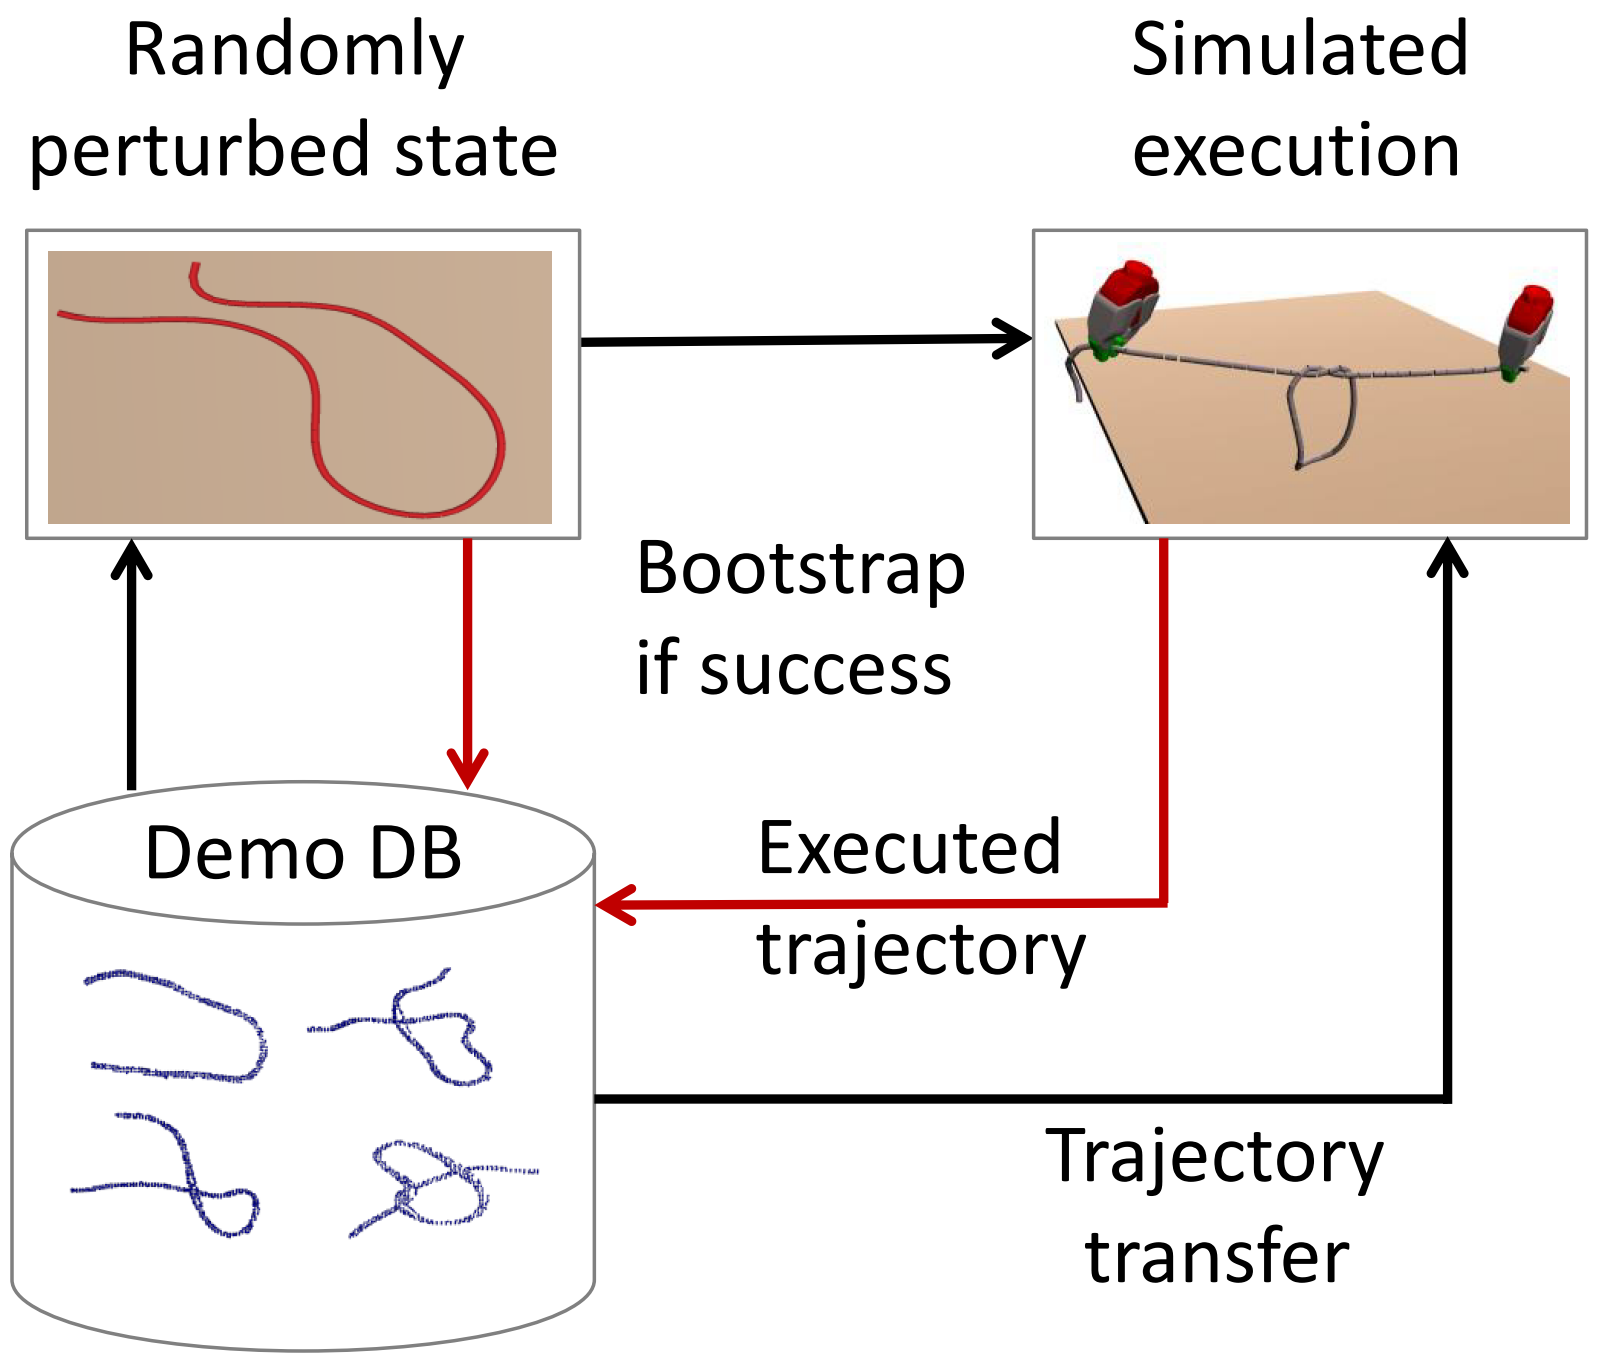
\includegraphics[width=\linewidth]{figs/teaser.png}
  \caption{Diagram of the bootstrapping approach we employ. Our system uses simulation
           of perturbed states from our demonstration set to augment a library of expert
           demonstrations. We find that this approach can leverage synthetic data to improve
           on the applicable of expert demonstrations by better modelling of states that
           trajectories can transfer to and allowing our approach to penalize less for
           transformations where transfer succeeds.}
  \label{fig:knot_steps}
\end{figure}




